% !TeX program = lualatex
% !TeX encoding = utf8
% !TeX spellcheck = uk_UA
% !BIB program = bibler

\documentclass[onlytextwidth]{beamer}
\usetheme{Electromagnetism}
\usepackage{Electromagnetism}
\usepackage{circuitikz}


%============================================================================
\title[Лекції електрики та магнетизму]{\huge\bfseries Енергія електричного поля}
\subtitle{Лекції з електрики та магнетизму}
\author{Пономаренко С. М.}
\date{}
%============================================================================
\graphicspath{{pictures/}}
\begin{document}
\begin{frame}[plain]
	\maketitle
\end{frame}

% ============================== Слайд ## ===================================
\begin{frame}{Зміст}{}
	\tableofcontents
\end{frame}
% ===========================================================================



%% --------------------------------------------------------
\section{Електрична ємність}
%% --------------------------------------------------------

% ============================== Слайд ## ===================================
\begin{frame}{Ємність провідника}{}\small
	\begin{block}{}\justifying
		Якщо провідник має заряд $q$, то його потенціал дорівнює $\phi$.

		\medskip

		Якщо заряд збільшити в $n$ разів, то через принцип суперпозиції в $n$ разів збільшиться і
		робота по переміщенню пробного заряду в полі провідника від його поверхні на нескінченність. Це
		означає, що в $n$ разів зросте і потенціал. Отже, відношення $q/\phi$ не повинно залежати від
		заряду провідника і характеризує сам провідник.

		\medskip

		Відповідно можна ввести \alert{ємність провідника} як: $\tcbhighmath{C= \frac{q}{\phi}.}$
	\end{block}

	\begin{block}{}\justifying
		Якщо маємо систему двох провідників. Нанесемо на один провідник заряд ($-q$), а на інший --- заряд
		($+q$). Різниця потенціалів провідників $\phi_+ - \phi_-$ пропорційна заряду $q$.

		\bigskip

		Ємність (\alert{взаємна ємність}) пари провідників визначається співвідношенням:
		$\tcbhighmath{C=
				\frac{q}{\phi_+ - \phi_-}.}$
	\end{block}
\end{frame}
% ===========================================================================



% ============================== Слайд ## ===================================
\begin{frame}{Конденсатори}{}\justifying
	\begin{block}{}
		Конденсатор складається з двох металевих пластин --- електродів, які називаються також
		\alert{обкладками}, між якими знаходиться тонкий шар діелектрика.
		\begin{columns}
			\begin{column}{0.6\linewidth}
				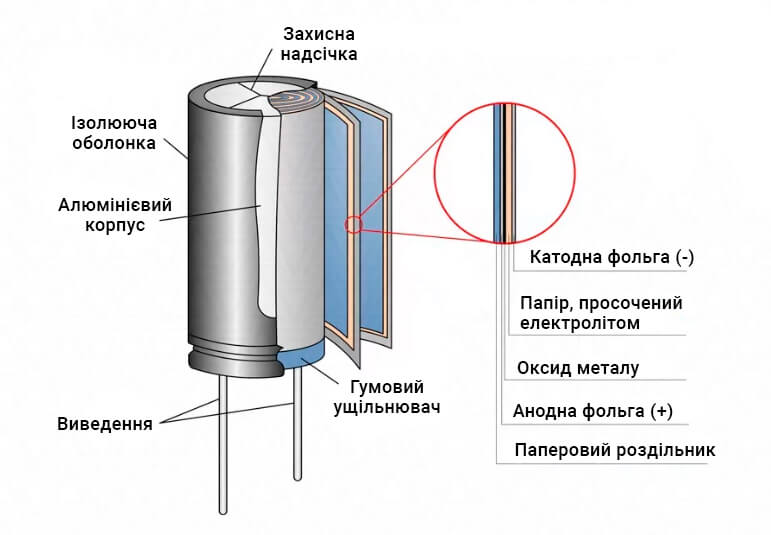
\includegraphics[width=\linewidth]{condensator}
			\end{column}
			\begin{column}{0.4\linewidth}
				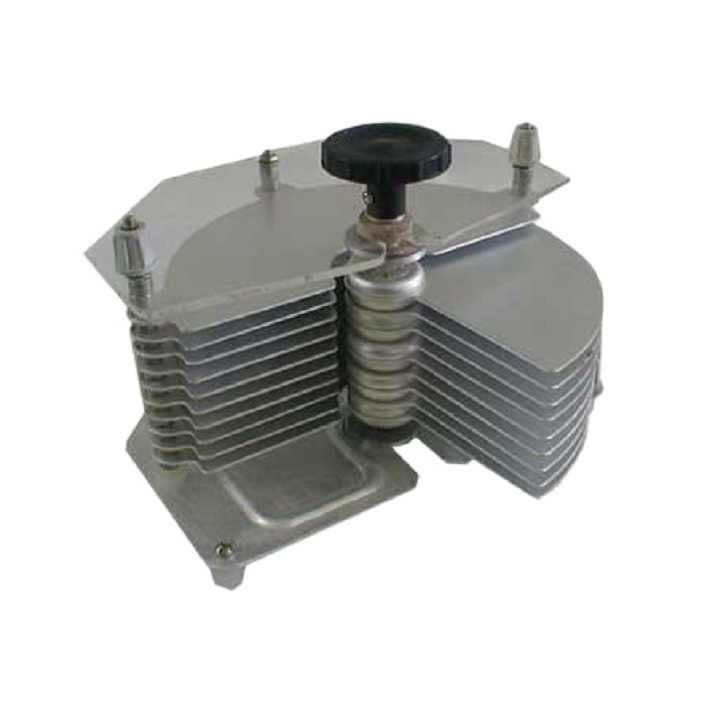
\includegraphics[width=\linewidth]{varcap}
			\end{column}
		\end{columns}
	\end{block}
	\begin{block}{}
		\href{https://www.youtube.com/watch?v=HmbwM8cM1FU&ab_channel=UW-MadisonPhysicsLectureDemonstrations}{\color{blue}Відео:
			Заряд та розряд конденсатора}
	\end{block}
\end{frame}
% ===========================================================================




% ============================== Слайд ## ===================================
\begin{frame}{З'єднання конденсаторів}{}
	\begin{columns}\centering
		\begin{column}{0.5\linewidth}\centering
			\begin{block}{}\small\centering
				Послідовне з'єднання
			\end{block}
		\end{column}
		\begin{column}{0.5\linewidth}\centering
			\begin{block}{}\small\centering
				Паралельне з'єднання
			\end{block}
		\end{column}
	\end{columns}
	\begin{columns}
		\begin{column}{0.5\linewidth}\centering
			\begin{circuitikz}[>=latex]
				% Послідовне з'єднання конденсаторів
				\draw (0,0)
				node[xshift=5pt, above, font=\tiny, text=red] {$+q$}
				to[C=$C_1$]
				node[above, font=\tiny, text=blue] {$-q$}
				++(1,0)
				node[xshift=5pt, above, font=\tiny, text=red] {$+q$}
				to[C=$C_2$]
				node[above, font=\tiny, text=blue] {$-q$}
				++(1,0)
				node[xshift=5pt, above, font=\tiny, text=red] {$+q$}
				to[C=$C_3$]
				node[above, font=\tiny, text=blue] {$-q$}
				++(1,0)
				node[right] {\ldots} ++(0.5,0)
				node[xshift=5pt, above, font=\tiny, text=red] {$+q$}
				to[C=$C_n$]
				node[above, font=\tiny, text=blue] {$-q$}
				++(1,0) coordinate (C) node[circle, fill, inner sep=1pt] {} ;
				\draw (0,0) node[circle, fill, inner sep=1pt] {} -- ++(0, -1);
				\draw (C) -- ++(0, -1);
				\draw[<->] ([yshift=-0.75cm]0,0)  -- node[below,
					font=\scriptsize] {$U = U_1+U_2
						+U_3 + \ldots +
						U_n$}
				([yshift=-0.75cm]C);
			\end{circuitikz}
		\end{column}
		\begin{column}{0.5\linewidth}\centering
			\begin{circuitikz}[>=latex, scale=0.6, transform shape]
				% Верхня лінія
				\foreach \y in {1,...,5} {
						\ifnum\y=4
							\node at (1,{1.5*\y}) {$\ldots$};
						\else
							\ifnum\y=5
								\edef\c{n}
							\else
								\edef\c{\y}
							\fi
							\draw (0, {1.5*\y}) to[C=$C_\c$] ++(2,0);
						\fi

					}
				\draw[red, thick] (0,1.5) -- ++(0,{4*1.5});
				\draw[blue, thick]  (2,1.5) -- ++(0,{4*1.5});

				\draw[thick, red] (-1, {3*1.5}) node[circle, fill, inner sep=1pt] (A) {} -- ++(1,
				0) ;
				\draw[thick, blue] (2, {3*1.5})   -- ++(1, 0) node[circle, fill,
					inner sep=1pt] (B) {} ;

				\draw[] (A) -- ++(0, -4) coordinate (D) ;
				\draw[] (B) -- ++(0, -4) coordinate (E);
				\draw[<->] ([yshift=0.25cm]D) -- node[below] {$U$} ([yshift=0.25cm]E);

				\fill[opacity=0.2, dashed, red!40,  very thin] (-0.55,1) rectangle ++(1.5, 7);
				\fill[opacity=0.2, dashed, blue!40, very thin] (1.05,1) rectangle ++(1.5, 7);
			\end{circuitikz}

		\end{column}
	\end{columns}
	\begin{columns}
		\begin{column}{0.5\linewidth}
			\begin{equation*}
				\frac1C = \sum\limits_{i = 1}^n \frac1{C_i}.
			\end{equation*}
		\end{column}
		\begin{column}{0.5\linewidth}
			\begin{equation*}
				C = \sum\limits_{i = 1}^n {C_i}.
			\end{equation*}
		\end{column}
	\end{columns}
\end{frame}
% ===========================================================================

% ============================== Слайд ## ===================================
\begin{frame}{Задачі}{}\scriptsize
	\begin{exampleblock}{\scriptsize Задача 1}
		Знайдіть ємність сферичного провідника радіусом $R$.
	\end{exampleblock}
	\begin{exampleblock}{\scriptsize Задача 2}
		Знайдіть ємність плоского конденсатора, відстань між обкладками якого дорівнює $d$,
		площа пластин $S$, простір заповнено діелектриком з проникністю $\epsilon$.

		\bigskip

		Відповідь: $C = \frac{\epsilon S}{4\pi d}$.
	\end{exampleblock}
	\begin{exampleblock}{\scriptsize Задача 3}
		Знайдіть ємність сферичного конденсатора, радіуси обкладок $R_1$ та $R_2$, простір
		заповнено діелектриком з проникністю $\epsilon$.

		\bigskip

		Відповідь: $C = \frac{\epsilon R_1R_2}{R_2 - R_1}$.
	\end{exampleblock}
	\begin{exampleblock}{\scriptsize Задача 4}
		Знайдіть ємність циліндричного конденсатора висотою $\ell$, радіуси обкладок $R_1$ та
		$R_2$, простір
		заповнено діелектриком з проникністю $\epsilon$.

		\bigskip

		Відповідь: $C = \frac{\epsilon \ell}{2\ln\frac{R_1}{R_2} d}$.
	\end{exampleblock}
\end{frame}
% ===========================================================================




% ============================== Слайд ## ===================================
\begin{frame}{Взаємна ємність двох куль}{}
	\begin{exampleblock}{\scriptsize Задача 5}\scriptsize\justifying
		Знайдемо (взаємну) ємність системи з двох металевих тіл (куль), що мають власні ємності
		$C_1$ і $C_2$ і перебувають на відстані $d$ одна від одної, вважаючи $d \gg C_1,C_2$.
		Останнє означає, що одна відносно одної кулі можна вважати точковими.
	\end{exampleblock}
	\begin{center}
		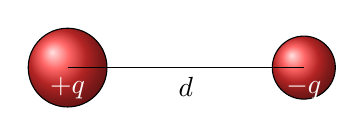
\begin{tikzpicture}[]
			\coordinate (+q)  at (0,0);
			\coordinate (-q)  at (3,0);
			\draw[ball color = red!80] (+q) circle (0.5) node[below, text=white] {$+q$};
			\draw[ball color = red!80] (-q) circle (0.4) node[below, text=white] {$-q$};
			\draw (+q) -- node[below] {$d$} (-q);
		\end{tikzpicture}
	\end{center}
	\begin{block}{\scriptsize Розв'язок}\scriptsize\justifying
		Нанесемо заряд $+q$ на кулю ємністю $C_1$ і заряд $-q$ на кулю ємністю $C_2$. Запишемо
		потенціали кульок з урахуванням їхнього взаємного впливу:
		\begin{equation*}
			\begin{cases}
				\phi_+ = \frac{q}{C_1} - \frac{q}{b}, \\
				\phi_- = -\frac{q}{C_1} + \frac{q}{b}.
			\end{cases}
		\end{equation*}
		Різниця потенціалів $\phi_+ - \phi_- = q\left( \frac1{C_1} + \frac1{C_2} - \frac2d\right) $, а
		ємність системи:
		\begin{equation*}
			C = \frac{q}{\phi_+ - \phi_-} \approx \frac{C_1C_2}{C_1 + C_2} \left(1 + \frac{C_1C_2}{C_1 +
				C_2}\frac2{d} \right) .
		\end{equation*}
	\end{block}
\end{frame}
% ===========================================================================


%% --------------------------------------------------------
\section{Енергія електричного поля}
%% --------------------------------------------------------

% ============================== Слайд ## ===================================
\begin{frame}{Взаємна енергія системи зарядів}\small
	\begin{columns}
		\begin{column}{0.8\linewidth}
			\begin{block}{}\justifying
				Щоб зблизити два заряди $q_1$ і $q_2$ до відстані $r_{12}$, потрібно здійснити
				роботу проти сил поля $A = \frac{q_1q_2}{r_{12}}$, тобто, пара зарядів, яку ми
				розглядаємо, має енергію $ U = \frac{q_1q_2}{r_{12}} $.
			\end{block}
		\end{column}
		\begin{column}{0.2\linewidth}\centering

			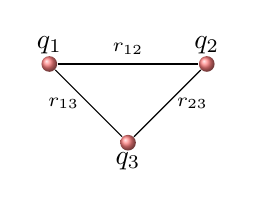
\begin{tikzpicture}[]
				\node[circle, ball color=red!50, inner sep=2 pt] (q1) at (0, 0) {}; \node[above] at
				(q1)
				{$q_1$};
				\node[circle, ball color=red!50, inner sep=2 pt] (q2) at (2, 0) {}; \node[above] at
				(q2)
				{$q_2$};
				\node[circle, ball color=red!50, inner sep=2 pt] (q3) at (1, -1) {}; \node[below]
				at (q3)
				{$q_3$};
				\draw (q1) -- node[above, font=\scriptsize] {$r_{12}$} (q2);
				\draw (q1) -- node[left, font=\scriptsize] {$r_{13}$} (q3);
				\draw (q2) -- node[right, font=\scriptsize] {$r_{23}$} (q3);
			\end{tikzpicture}
		\end{column}
	\end{columns}
	\begin{block}{}
		Для системи зарядів взаємна енергія дорівнює:
		$
			U = \frac12\sum\limits_{i = 1}^n\sum\limits_{\stackrel{j = 1}{i \neq j}}^n
			\frac{q_iq_j}{r_{ij}}
		$.
	\end{block}
	\begin{block}{}\justifying
		Потенціал поля в точці знаходження $i$-го заряду, створюваний усіма зарядами (крім $i$-го):
		\begin{equation*}
			\phi_i = \sum\limits_{\stackrel{j = 1}{i \neq j}}^n \frac{q_j}{r_{ij}}.
		\end{equation*}
		Потенціальна енергія всієї системи зарядів:
		\begin{equation*}
			W = \frac12\sum_iq_i\sum\limits_{\stackrel{j = 1}{i \neq j}}^n \frac{q_j}{r_{ij}} =
			\frac12
			\sum_i q_i\phi_i
		\end{equation*}
	\end{block}
\end{frame}
% ===========================================================================


% ============================== Слайд ## ===================================
\begin{frame}{Електростатична енергія тіл}
	\begin{center}
		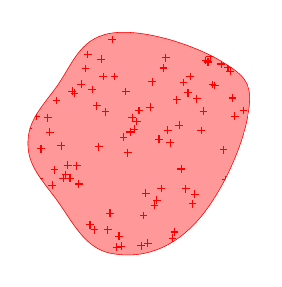
\begin{tikzpicture}[>=latex,
				charge/.style = {ball color=red!50, font=\scriptsize, inner sep=1pt},
				surface/.style = {draw, opacity=0.5, smooth cycle, tension=.7},
				filled_surface/.style = {red, fill=red!50, smooth cycle, tension=.7},
				>=latex,
				scale=0.7,
				transform shape
			]
			\def\coordinates{
				(-1,0)
				(-0.5,1)
				(0.5,2)
				(2.5,1.5)
				(3,0.5)
				(2,-1.5)
				(0.5,-2)
				(-0.5,-1)
			}
			\begin{scope}
				\clip[yshift=2cm] plot[smooth cycle, tension=.7] coordinates \coordinates;
				\draw[yshift=2cm, draw=red, fill=red!40] plot[smooth cycle, tension=.7]
				coordinates \coordinates;
				\draw plot [only marks, mark=+, domain=-1:3, samples=100, mark
				options={color=red}]
				(\x,{rnd*4});
			\end{scope}
		\end{tikzpicture}
	\end{center}
	\begin{block}{}\justifying
		Якщо заряди розподілені в просторі з об'ємною густиною $\rho(\vect{r})$, а також на
		поверхнях
		--- з поверхневою густиною $\sigma(\vect{r})$, формула
		\begin{equation*}
			W = \sum_i q_i\phi_i
		\end{equation*}
		узагальнюється як:
		\begin{equation*}
			\tcbhighmath{W = \frac12 \iiint\limits_V \rho(\vect{r})\phi(\vect{r}) dV + \frac12
				\iint\limits_S
				\sigma(\vect{r})\phi(\vect{r}) dS.}
		\end{equation*}
	\end{block}
\end{frame}
% ===========================================================================


% ============================== Слайд ## ===================================
\begin{frame}{Задачі}{}
	\begin{exampleblock}{\scriptsize Задача 1}\justifying\scriptsize
		Нехай куля радіуса $R$ несе повний заряд $Q$, що рівномірно розподілений по поверхні.
		Знайти електростатичну енергію кулі.
	\end{exampleblock}
	\begin{block}{\scriptsize Розв'язок}\justifying\scriptsize
		Енерргію знайдемо як:
		\begin{equation*}
			W =  \frac12 \iint\limits_S \sigma(\vect{r})\phi(\vect{r}) dS =
			\frac12\sigma\frac{Q}{R}4\pi
			R^2 = \frac{Q^2}{2R}
		\end{equation*}
	\end{block}

	\begin{exampleblock}{\scriptsize Задача 2}\justifying\scriptsize
		Нехай куля радіуса $R$ несе повний заряд $Q$, що рівномірно розподілений по об'єму.
		Знайти електростатичну енергію кулі.

		\bigskip

		Відповідь: $W = \frac35 \frac{Q^2}{R}$
	\end{exampleblock}

	\begin{alertblock}{}\centering
		Де локалізована енергія поля?
	\end{alertblock}
\end{frame}
% ===========================================================================


% ============================== Слайд ## ===================================
\begin{frame}{Енергія електричного поля в конденсаторі}{}\small
	\begin{columns}
		\begin{column}{0.8\linewidth}
			\begin{block}{}\justifying
				Зарядимо конденсатора за допомогою перенесення заряду з правої пластини на ліву. Робота з
				перенесення заряду $dq$ дорівнює $dW = \Delta\phi dq$, де $\Delta\phi$ --- різниця
				потенціалів пластин. Оскільки $\phi = \frac{q}{C}$, то енергія буде дорівнювати:
				\begin{equation*}
					dW = \Delta\phi dq = \frac{qdq}{C}\ \Rightarrow\ W = \frac{q^2}{2C} =
					\frac{C\Delta\phi^2}{2}.
				\end{equation*}
			\end{block}
		\end{column}
		\begin{column}{0.2\linewidth}\centering
			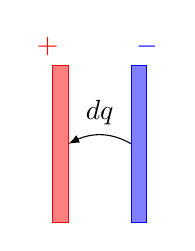
\begin{tikzpicture}[>=latex]
				\draw[red, fill=red!50] (0,0) rectangle ++(0.2,2)  node[above left] {$+$};
				\draw[blue, fill=blue!50] (1,0) rectangle ++(0.2,2) node[above] {$-$};
				\draw[<-] (0.2, 1) to[bend left] node[above] {$dq$} ++(0.8,0);
			\end{tikzpicture}
		\end{column}
	\end{columns}
	\begin{overprint}
		\onslide<1>
		\begin{block}{}
			В плоскому конденсаторі поле однорідне $\Delta\phi = Ed$, ємність плоского конденсатора $C =
				\frac{\epsilon S}{4\pi d}$, то для енергії конденсатора отримуємо:
			\begin{equation*}
				W = \frac12 C\Delta\phi^2 = \frac12 \frac{\epsilon S}{4\pi d} (Ed)^2 =
				\frac{\epsilon
					E^2}{8\pi}V.
			\end{equation*}
			де $V = Sd$  --- об'єм конденсатора. Густина енергії дорівнює
			\begin{equation*}
				w = \frac{\epsilon
					E^2}{8\pi}, \quad\ \text{якщо}\ D = \epsilon E\ \Rightarrow\ w = \frac{ED}{8\pi}.
			\end{equation*}
		\end{block}
		\onslide<2>
		\begin{block}{}\justifying
			Енергія конденсатора виражена через характеристики поля (а не заряди):
			\begin{equation*}
				w = \frac{ED}{8\pi}
			\end{equation*}
			що дозволяє дати нову інтерпретацію результату. Переносником взаємодії зарядів є \alert{електричне
				поле}, так що воно і  \alert{є носієм енергії}, передає енергію від одного заряду до іншого.
			Електричне поле присутнє тільки в об'ємі конденсатора, тож і його \alert{енергія локалізована в тих
				областях простору, де присутнє поле}.
		\end{block}
	\end{overprint}
\end{frame}
% ===========================================================================


% ============================== Слайд ## ===================================
\begin{frame}{Енергія електричного поля (загальне виведення)}{}\scriptsize
	\begin{block}{}\justifying
		Отримана формула для енергії електричного поля для окремого випадку, коли поле однорідне і
		локалізоване в конденсаторі. Наведемо тепер більш загальний висновок.
	\end{block}
	\begin{block}{}
		При зміні заряду системи на $\delta\rho$, енергія змінюється на величину
		\begin{equation*}
			\delta W = \frac12 \iiint\limits_V \delta\rho(\vect{r})\phi(\vect{r}) dV.
		\end{equation*}
		З теореми Гаусса $\delta\rho = \frac1{4\pi}\Div\delta\Dfield$:
		\begin{equation*}
			\delta W = \frac1{8\pi} \iiint\limits_V \frac1{4\pi}\Div\delta\Dfield \phi dV =
			\frac1{8\pi} \iiint\limits_V \left( \Div(\delta\Dfield \phi) -
			\delta\Dfield\cdot\vect{\nabla}\phi\right) .
		\end{equation*}
	\end{block}
	\begin{alertblock}{}\tiny
		Інтегрування поширене на весь нескінченний простір. Але на великій відстані від системи зарядів
		поле обертається в нуль. Тому,перший доданок у правій частині $\iiiint\limits_V \left(
			\Div(\delta\Dfield \phi\right) dV = \oiint\limits_{S\to\infty} (\phi\delta\Dfield)\cdot
			d\vect{S} =
			0$
	\end{alertblock}
	\begin{block}{}
		У другому доданку врахуємо зв'язок потенціалу та напруженості поля: $\Efield = -
			\vect{\nabla}\phi$:
		\begin{equation*}
			\delta W =
			\iiint\limits_V
			\frac{\Efield\cdot \delta\Dfield}{{8\pi}} dV,\ \Rightarrow\ w = \frac{\Efield\cdot
				\delta\Dfield}{{8\pi}}.
		\end{equation*}
	\end{block}
\end{frame}
% ===========================================================================






% ============================== Слайд ## ===================================
\begin{frame}{Власна та взаємна енергія зарядів}{}\small
	\begin{columns}
		\begin{column}{0.5\linewidth}\centering
			Взаємна енергія зарядів:
		\end{column}
		\begin{column}{0.5\linewidth}\centering
			Енергія поля:
		\end{column}
	\end{columns}
	\begin{columns}
		\begin{column}{0.5\linewidth}
			\begin{equation*}
				W = \frac12 \sum \frac{q_iq_j}{r_{ij}}.
			\end{equation*}
		\end{column}
		\begin{column}{0.5\linewidth}
			\begin{equation*}
				W = \int\limits_V \frac{E^2}{8\pi} dV.
			\end{equation*}
		\end{column}
	\end{columns}
	\begin{alertblock}{}\justifying
		Формула ліворуч може бути як додатною так і від'ємною.  Формула праворуч дає значення енергії
		завжди позитивне, оскільки містить інтеграл від невід'ємної величини.
	\end{alertblock}
	\begin{block}{}
		Поле системи двох зарядів $\Efield = \Efield_1 + \Efield_2$ має енергію:
		\begin{equation*}
			W = \int\limits_V \frac{E^2}{8\pi} dV = \int\limits_V \frac{(\Efield_1 +
				\Efield_2)^2}{8\pi} dV = \int\limits_V \frac{E_1^2}{8\pi} dV + \int\limits_V \frac{E_2^2}{8\pi}
			dV + \int\limits_V \frac{\Efield_1\Efield_2}{8\pi} dV
		\end{equation*}
	\end{block}
	\begin{columns}
		\begin{column}{0.5\linewidth}\centering
			Власна енергія зарядів:
		\end{column}
		\begin{column}{0.5\linewidth}\centering
			Взаємна енергія:
		\end{column}
	\end{columns}
	\begin{columns}
		\begin{column}{0.5\linewidth}
			\begin{equation*}
				\int\limits_V \frac{E_1^2}{8\pi} dV > 0, \int\limits_V \frac{E_2^2}{8\pi} dV >0.
			\end{equation*}
		\end{column}
		\begin{column}{0.5\linewidth}
			\begin{equation*}
				W_\text{вз} = \int\limits_V \frac{\Efield_1\Efield_2}{8\pi} dV \lesseqgtr 0.
			\end{equation*}
		\end{column}
	\end{columns}
\end{frame}
% ===========================================================================


%% --------------------------------------------------------
\section{Пондеромоторні сили}
%% --------------------------------------------------------


% ============================== Слайд ## ===================================
\begin{frame}{Енергетичний метод обчислення сил}{Теорія}
	\begin{onlyenv}<1>
		\begin{block}{}\justifying
			Одним з ефективних прийомів розрахунку сил є \alert{метод віртуальних переміщень}, у якому
			обчислюють роботу сил поля $\delta A = F dx$ у разі нескінченно малого зсуву $dx$, після
			чого сила знаходиться з рівності $ F = \delta A / dx $.

			\bigskip

			Метод є універсальним, без вияснення причин виникнення сил і автоматично враховувати всі
			силові взаємодії (електричні та механічні).
		\end{block}
	\end{onlyenv}
	\begin{onlyenv}<2>\small
		\begin{block}{}\justifying
			Нехай на провідниках підтримуються постійними заряди, $q = \const$, тобто немає зовнішніх
			джерел енергії.
		\end{block}
		\begin{block}{}\justifying
			За таких умов робота $\delta A$ всіх внутрішніх сил системи під час віртуальних переміщень
			провідників і діелектриків відбувається за рахунок зменшення електричної енергії $dW$ системи:
			$
				\delta A = - \left( dW\right)_{q=\const}.
			$
		\end{block}
		\begin{block}{}\scriptsize
			Нехай нас цікавить сила, що діє на дане тіло (провідник або діелектрик). Зробимо нескінченно
			мале поступальне переміщення $dx$ цього тіла в цікавому для нас напрямку $x$. Тоді робота
			шуканої сили $F_x$ визначиться як $\delta A = F_x dx$, звідки:
			\begin{equation*}
				\tcbhighmath{F_x = -\left.\frac{dW}{dx}\right|_{q=\const}.}
			\end{equation*}
		\end{block}
		\begin{alertblock}{}\scriptsize
			Для обчислення сили за цією формулою не треба підбирати такий режим, за якого обов'язково всі
			заряди провідників залишалися б постійними. Треба просто знайти приріст $dW$ за умови, що $q =
				\const$ --- це суто математична операція.
		\end{alertblock}
	\end{onlyenv}
	\begin{onlyenv}<3>\small
		\begin{columns}
			\begin{column}{0.6\linewidth}
				\begin{block}{}\justifying
					Нехай тепер на провідниках підтримуються постійними потенціали $\phi=\const$.
					Для цього всистемі є \alert{джерело, що постачає заряди і витрачають енергію на
						здійснення роботи}. Із закону збереження енергії, робота джерела йде на
					виконання механічної роботи $F_x dx$ та на зміну енергії поля $dW$:
					\begin{equation*}
						\delta A_\text{дж} = F_x dx + dW
					\end{equation*}
				\end{block}
			\end{column}
			\begin{column}{0.4\linewidth}
				\begin{circuitikz}[]
					\draw
					(0,0) to[battery1, l=$\Delta\phi$] (0,2)
					-- (1.5,2) to[C, l=$C$, color=red] (1.5,0) -- (0,0);
				\end{circuitikz}
			\end{column}
		\end{columns}
		\begin{block}{}\justifying
			З іншого боку робота джерела по переміщенню заряду дорівнює $\delta A_\text{дж} =
				\delta q \Delta\phi = \Delta\phi^2 \delta C$, а $dW = \frac12 \Delta\phi^2 \delta C $,
			звідки $   F_xdx =  \frac12 \Delta\phi^2 \delta C = dW$, тобто:
			\begin{equation*}
				\tcbhighmath{F_x = +\left.\frac{dW}{dx}\right|_{\Delta\phi=\const}.}
			\end{equation*}
		\end{block}
		%		\begin{alertblock}{}\scriptsize
		%			Для обчислення сили за цією формулою не треба підбирати такий режим, за якого
		%			потенціали постійні. Треба просто знайти приріст $dW$ за умови, що $\Delta\phi =
		%				\const$ --- це знову ж суто математична операція.
		%		\end{alertblock}
	\end{onlyenv}
\end{frame}
% ===========================================================================




% ============================== Слайд ## ===================================
\begin{frame}{Енергетичний метод обчислення сил}{Приклади}\small
	\begin{exampleblock}{Приклад 1}\justifying
		Знайдемо силу тяжіння пластин зарядженого конденсатора.
	\end{exampleblock}

	\begin{columns}
		\begin{column}{0.8\linewidth}
			\begin{block}{}\justifying
				За умов, коли пластини конденсатора нерухомі, сила їхнього притягання не залежить
				від способу обчислення.
			\end{block}
		\end{column}
		\begin{column}{0.2\linewidth}
			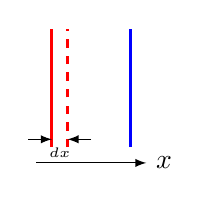
\begin{tikzpicture}[>=latex]
    \pgfmathsetmacro{\h}{1.5}
    \pgfmathsetmacro{\d}{1}
    \pgfmathsetmacro{\D}{0.2}
	\draw[line width=1pt, red] (0, 0) -- ++(0, \h);
	\draw[line width=1pt, red, dashed] (\D, 0) -- ++(0, \h);
	\draw[line width=1pt, blue] (\d, 0) -- ++(0, \h);
	\draw[->] (-\D, -\D) -- ++({\d + 2*\D},0) node[right] {$x$};
	\draw[->] (-0.3, 0.1) -- (0, 0.1);
	\draw[->] (0.5, 0.1) -- (0.2, 0.1);
	\node[below, font=\tiny, inner sep=0] at (0.1,0) {$dx$};
\end{tikzpicture}
		\end{column}
	\end{columns}
	\begin{onlyenv}<1>
		\begin{block}{}\justifying
			Обчислимо силу у випадку $q = \const$.
			Зміна енергії поля при зміні відстані між пластинами:
			\begin{equation*}
				dW = d\left(\frac{q^2}{2C} \right)  = -\frac{q^2}{2C^2} dC, \quad C = \frac{\epsilon
					S}{4\pi
					x}, \quad dC = -\frac{C}{x} dx\ \Rightarrow\ dW = \frac{q^2}{2C x} dx.
			\end{equation*}
			\begin{equation*}
				dW = \frac{\Delta\phi^2 C}{2d} dx = \frac{E^2\cancel{d^2} \epsilon S}{2\cancel{d}\ 4\pi
					\cancel{d}} dx,
				\quad F_x = -\frac{dW}{dx} = -\frac{\epsilon E^2}{8\pi} S
			\end{equation*}
			\alert{\scriptsize Знак <<мінус>> свідчить про те, що пластини притягуються одна до одної.}
		\end{block}
	\end{onlyenv}
	\begin{onlyenv}<2>
		\begin{block}{}\justifying
			Обчислимо силу у випадку $\Delta\phi = \const$. Зміна енергії поля при зміні відстані між
			пластинами:
			\begin{equation*}
				dW = d\left(\frac{C \Delta\phi^2}{2} \right)  = \frac{\Delta\phi^2}{2} dC,\ C =
				\frac{\epsilon S}{4\pi
					x},\ dC = -\frac{C}{x} dx\ \Rightarrow\ dW = -\frac{\Delta\phi^2 C}{2x} dx.
			\end{equation*}
			\begin{equation*}
				dW = -\frac{\Delta\phi^2 C}{2d} dx = -\frac{E^2\cancel{d^2} \epsilon
				S}{2\cancel{d}\ 4\pi
					\cancel{d}} dx,
				\quad F_x = \frac{dW}{dx} = -\frac{\epsilon E^2}{8\pi} S
			\end{equation*}
			\alert{\scriptsize Знак <<мінус>> свідчить про те, що пластини притягуються одна до одної.}
		\end{block}
	\end{onlyenv}
\end{frame}
% ===========================================================================


% ============================== Слайд ## ===================================
\begin{frame}{Енергетичний метод обчислення сил}{Приклади}\small
	\begin{exampleblock}{\href{https://www.youtube.com/watch?v=aBAdSE2jC8Y}{Приклад 2}}\justifying
		Знайдемо силу, з якою пластина з діелектрика з діелектричною проникністю $\epsilon$
		втягується в
		конденсатор.
	\end{exampleblock}
	\begin{columns}
		\begin{column}{0.6\linewidth}
			\begin{block}{\scriptsize Модель}\justifying\scriptsize
				Замінимо конденсатор із частково всунутою в нього пластиною діелектрика двома
				паралельно з'єднаними конденсаторами, з яких один --- вакуумний, а інший заповнений
				діелектриком.
			\end{block}
		\end{column}
		\begin{column}{0.4\linewidth}\centering
			\tikzset{pics/plate/.style n args={6}{
    % #1 thickness
    % #2 length
    % #3 angle
    % #4 width
    % #5 color
    code = {
        \draw[line join = round, #6, fill=#5] (0,-#1) coordinate (A) --
                                  ++(#2,0) coordinate (B) --
                                  ++(#3:#4) coordinate (C) --
                                  ++(-#2,0) coordinate (D) -- (A);
        \draw[line join = round, #6, fill=#5] (A) -- ++(0,-#1) coordinate (A1) --
                                  ++(#2,0) coordinate (B1) --
                                  (B) -- cycle;
        \draw[line join = round, #6, fill=#5] (B1) -- ++(#3:#4) coordinate (C1) --
                                  (C) -- (B) -- cycle;
    }
}}

\begin{tikzpicture}[>=latex, scale=0.8, transform shape]

\draw  (0,-1)    pic {plate={0.2}{3}{20}{1}{blue!10}{gray}};
\draw  (1.2,0.29)  pic {plate={0.73}{3}{20}{1}{gray!50}{gray}};
\draw  (0,0)     pic {plate={0.2}{3}{20}{1}{red!20}{gray}};

\draw[gray, <->] (1,0.3) -- node[above] {$L$} ++(3, 0);
\draw[gray, <->] (-0, -0.05) -- node[above] {$h$} ++(20:1);
\draw[gray, <->] (-0.1, -0.4) -- node[left] {$d$} ++(0, -0.8);
\draw[gray,  <-]  (0,-1.7) node[left] {$x$} -- ++(3,0) ;

\draw [red, decorate,decoration={brace,amplitude=5pt,raise=0ex, mirror}]
  (1.23,-1.2) -- ++(1.75,0) node[midway, yshift=-10pt]{$x$};

\draw[->, line width=2pt, red] (1.2,-0.75) -- ++(-0.75,0) node[left] {$F$};

\end{tikzpicture}
		\end{column}
	\end{columns}
	\begin{overprint}
		\onslide<1>
		\begin{block}{}
			Ємність системи з двох паралельно з'єднаних конденсаторів дорівнює:
			\begin{equation*}
				C = C_1 + C_2 = \frac{S_1}{4\pi d} + \frac{\epsilon S_2}{4\pi d}.
			\end{equation*}
			Сумарна площа пластин конденсаторів незмінна, і можна записати
			\begin{equation*}
				S = S_1 + S_2, S_1 = \left(1- \frac{x}{L} \right)S, S_2 = \frac{x}{L}S, S= Lh
			\end{equation*}
		\end{block}
		\onslide<2>
		\begin{block}{}
			\begin{equation*}
				C = \frac{S}{4\pi d}\left( 1 + (\epsilon -1)\frac{x}{L} \right)
			\end{equation*}
			\begin{equation*}
				F_x = -\frac{dW}{dx} = -\frac{dW}{dC}\frac{dC}{dx},\ \frac{dW}{dC} = -\frac{q^2}{2C^2},\
				\frac{dC}{dx} = \frac{S}{4\pi d} \frac{\epsilon -1}{L}.
			\end{equation*}
			\begin{equation*}
				F_x = \frac{q^2}{2C^2} \frac{S}{4\pi d} \frac{\epsilon -1}{L} \stackrel{q = CEd}{=}
				\frac{(\epsilon -1)E^2}{8\pi} hd.
			\end{equation*}
		\end{block}
	\end{overprint}
\end{frame}
% ===========================================================================




% ============================== Слайд ## ===================================
\begin{frame}{Підсумки}{}\small
\begin{onlyenv}<1>
\begin{block}{1. Електрична ємність}
        \begin{itemize}
            \item Ємність провідника: $ C = \frac{q}{\phi} $.
            \item Ємність пари провідників: $ C = \frac{q}{\Delta\phi} $.
            \item Послідовне з'єднання конденсаторів: $\frac1C = \sum\limits_{i = 1}^n\frac1{C_i}$.
            \item Паралельне з'єднання конденсаторів: $C = \sum\limits_{i = 1}^n{C_i}$.
            \item Ємність плоского конденсатора: $ C = \frac{\epsilon S}{4\pi d} $.
            \item Ємність сферичного конденсатора: $ C = \frac{\epsilon R_1 R_2}{R_2 - R_1} $.
            \item Ємність циліндричного конденсатора: $ C = \frac{\epsilon \ell}{2 \ln
            \frac{R_2}{R_1}} $.
        \end{itemize}
    \end{block}
\end{onlyenv}
\begin{onlyenv}<2>
    \begin{block}{2. Енергія електричного поля}
        \begin{itemize}
            \item Енергія системи зарядів: $
            			U = \frac12\sum\limits_{i = 1}^n\sum\limits_{\stackrel{j = 1}{i \neq j}}^n
            			\frac{q_iq_j}{r_{ij}}
            		$.
            \item Енергія системи зарядів через потенціал: $ W = \frac{1}{2} \sum_{i} q_i \varphi_i
            $.
            \item Енергія тіла $ W = \frac12 \iiint\limits_V \rho(\vect{r})\phi(\vect{r}) dV +
            \frac12
				\iint\limits_S
				\sigma(\vect{r})\phi(\vect{r}) dS $.
            \item Енергія електричного поля в конденсаторі: $ W = \frac{q^2}{2C} = \frac{C \Delta
            \varphi^2}{2} $
            \item Енергія через напруженість поля: $ W = \iiint\limits_V\frac{\varepsilon
            E^2}{8\pi} dV $
        \end{itemize}
    \end{block}
\end{onlyenv}
\begin{onlyenv}<3>
    \begin{block}{3. Пондеромоторні сили}
        \begin{itemize}
            \item Сила при \(q = \const\): $ F_x = - \left( \frac{dW}{dx} \right)_{q = \const} =
            + \left( \frac{dW}{dx} \right)_{\Delta\phi = \const}$.
            \item Сила втягування діелектрика в конденсатор: $	F_x = \frac{(\epsilon -1)E^2}{8\pi}
            S_\text{торця}.$
        \end{itemize}
    \end{block}
\end{onlyenv}
\end{frame}
% ===========================================================================


\end{document}
